\documentclass[conference]{IEEEtran}
\IEEEoverridecommandlockouts
% The preceding line is only needed to identify funding in the first footnote. If that is unneeded, please comment it out.
\usepackage{cite}
\usepackage{amsmath,amssymb,amsfonts}
\usepackage{algorithmic}
\usepackage{graphicx}
\usepackage{textcompthe_annotated_transformer}
\usepackage{xcolor}
\usepackage[backend=biber,
            sorting=none,   % Keine Sortierung
            doi=true,       % DOI anzeigen
            isbn=true,     % ISBN nicht anzeigen
            url=true,       % URLs anzeigen
            maxnames=6,     % Ab 6 Autoren et al. verwenden
            minnames=1,     % und nur den ersten Autor angeben
            style=numeric-comp,]{biblatex}
\addbibresource{literatur.bib}

\def\BibTeX{{\rm B\kern-.05em{\sc i\kern-.025em b}\kern-.08em
    T\kern-.1667em\lower.7ex\hbox{E}\kern-.125emX}}
\begin{document}

\title{Transformer gibt es nicht nur im Kino}


\author{\IEEEauthorblockN{Jonathan Arns}
\IEEEauthorblockA{\textit{Hochschule Mannheim} \\
Fakultät für Informatik\\
Paul-Wittsack-Str. 10\\
68163 Mannheim\\
jonathan.arns@stud.hs-mannheim.de}
}

\maketitle

%%%%%%%%%%%%%%%%%%%%%%%%%%%%%%%%% Document beginning %%%%%%%%%%%%%%%%%%%%%%%%%%%%%%%%%%%%%%

\begin{abstract}
abstract
\end{abstract}


\section{Einleitung}
Natural Language Processing (NLP), die Verarbeitung Menschlicher Sprache, ist ein Anwendungbereich für Machine Learning, der bereits erheblich von deep neural networks (DNN) profitiert hat. Die zwei dominanten Arten von DNN Architekturen dabei waren lange Zeit recurrent neural networks (RNN) und convolutional neural networks (CNN). \cite{comparative_study_cnn_rnn}

2017 stellten Vaswani et al. \cite{attention_is_all_you_need} mit dem Transformer eine neue DNN Architektur vor, die seitdem unter Anderem große Aufmerksamkeit durch die erfolgreiche Verwendung in OpenAIs GPT-2 und GPT-3 Modellen erlangte.

\section{Sequence to Sequence Learning}
Traditionell waren DNNs trotz ihrer hohen Flexibilität und Effektivität für viele Aufgaben beschränkt auf Probleme, deren Eingaben und Ausgaben sich sinvoll in Vektoren mit fester Länge codieren lassen, da neuronale Netze generell eine feste Anzahl an Eingabe- und Ausgabeneuronen haben. Das ist zwar für viele Klassifizierungsprobleme und in der Bildverarbeitung kein Problem, sehr wohl aber für beispielsweise NLP, da die Länge von Texten im Vorfeld nicht immer bekannt ist. \cite{sequence_to_sequence}

Dieses Problem wird mittels Sequence to Sequence (Seq2Seq) Learning gelöst, mit dessen Hilfe beliebig lange Sequenzen von Elementen als Eingabe in vollkommen andere Sequenzen, anderer Länge und aus anderen Elementen, transformiert werden können. \cite{sequence_to_sequence}

Die meisten Seq2Seq Modelle bestehen aus einem Encoder und einem Decoder \cite{attention_is_all_you_need}. Der Encoder codiert die Eingabe Sequenz in einer höher-dimensionale Vektorrepräsentation, die dann vom Decoder in eine Ausgabe Sequenz umgewandelt wird. Die Encoder und Decoder selbst sind in der Regel RNNs, beispielsweise mit der LSTM Architektur.


\section{Modell Architektur}

\begin{figure}[htbp]
\centerline{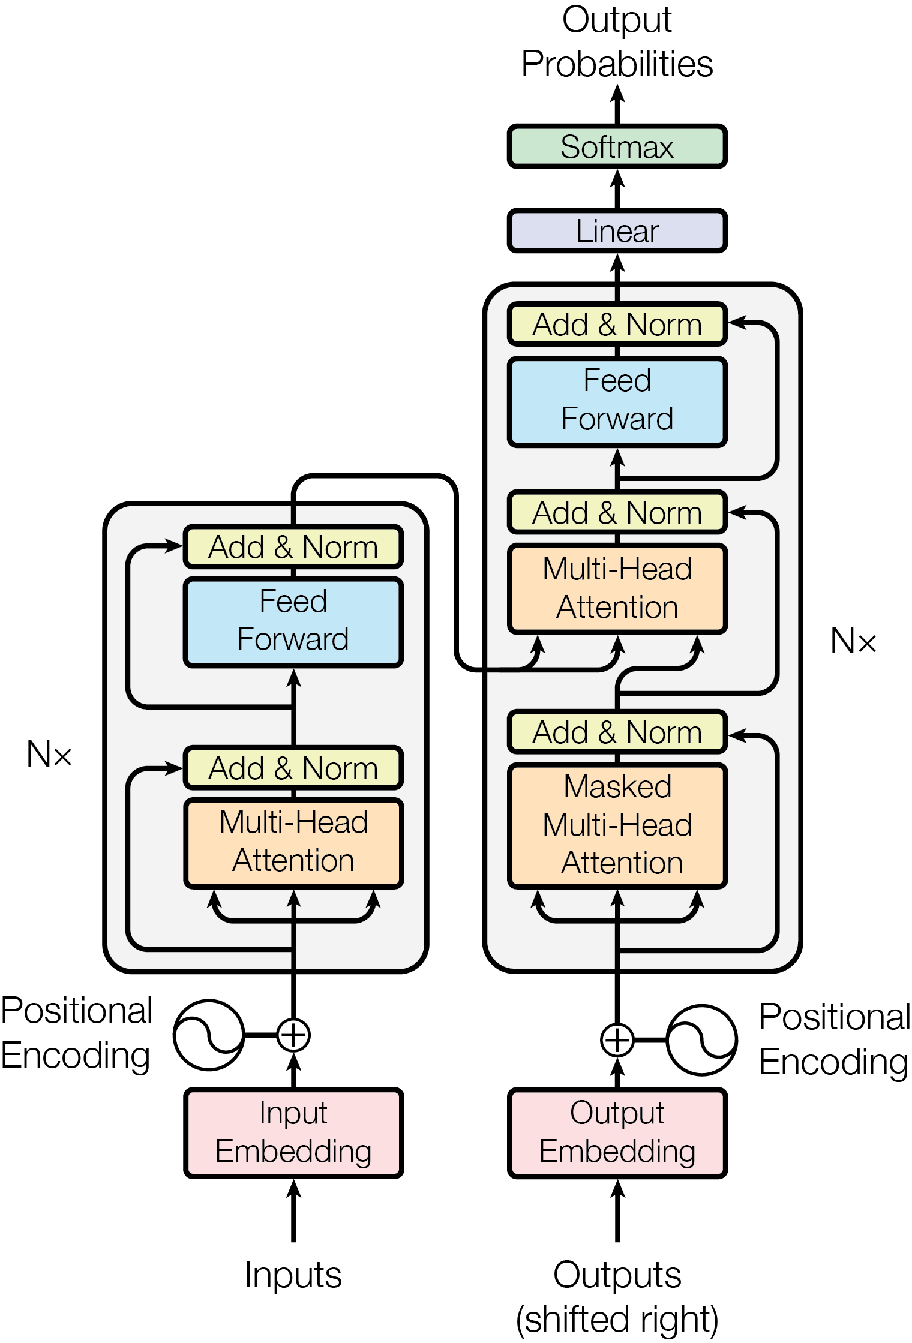
\includegraphics{img/figure1.png}}
\caption{Der Encoder (links) besteht aus einer Reihe von N identischen Modulen mit jeweils zwei Untermodulen. \\
Der Decoder (rechts) besteht auch aus einer Reihe von N identischen Modulen, jedoch mit jeweils drei Untermodulen. Die erste Schicht ist eine Multi-Head Attention Layer \cite{attention_is_all_you_need}}
\label{fig}
\end{figure}


\section{Attention}

\begin{figure}[htbp]
\centerline{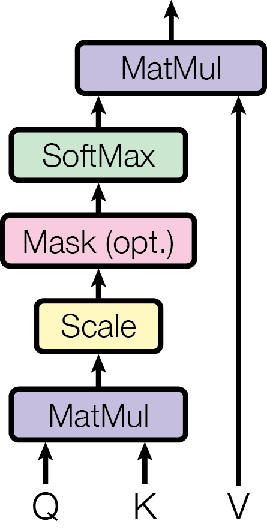
\includegraphics{img/scaled_dotproduct_attention.png}}
\caption{Scaled dotproduct attention \cite{attention_is_all_you_need}}
\label{fig}
\end{figure}

\begin{equation}
    Attention(Q,K,V) = softmax(\frac{QK^T}{\sqrt{d_K}})V
\end{equation}

\begin{figure}[htbp]
\centerline{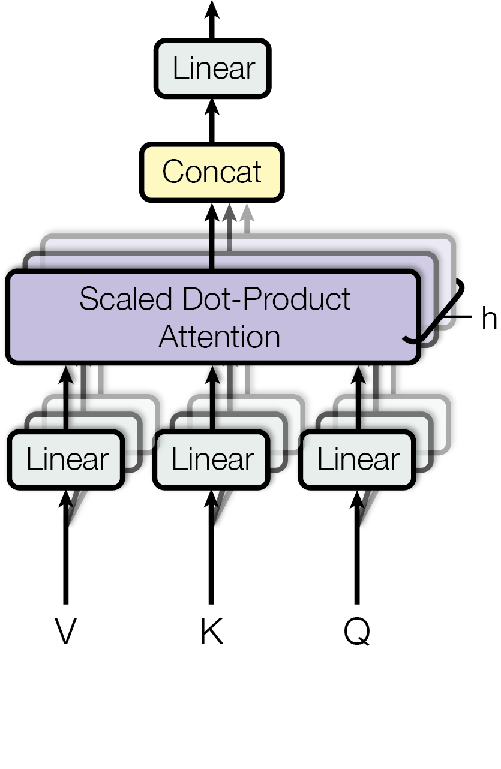
\includegraphics{img/multi_head_attention.png}}
\caption{Multi-Head Attention \cite{attention_is_all_you_need}}
\label{fig}
\end{figure}

\begin{eqnarray}
    MultiHead(Q,K,V) = Concat(head_1,...,head_h)W^O \\
    \text{mit} \; head_i = Attention(QW_i^Q , KW_i^K , VW_i^V)
\end{eqnarray}


\begin{figure}[htbp]
\centerline{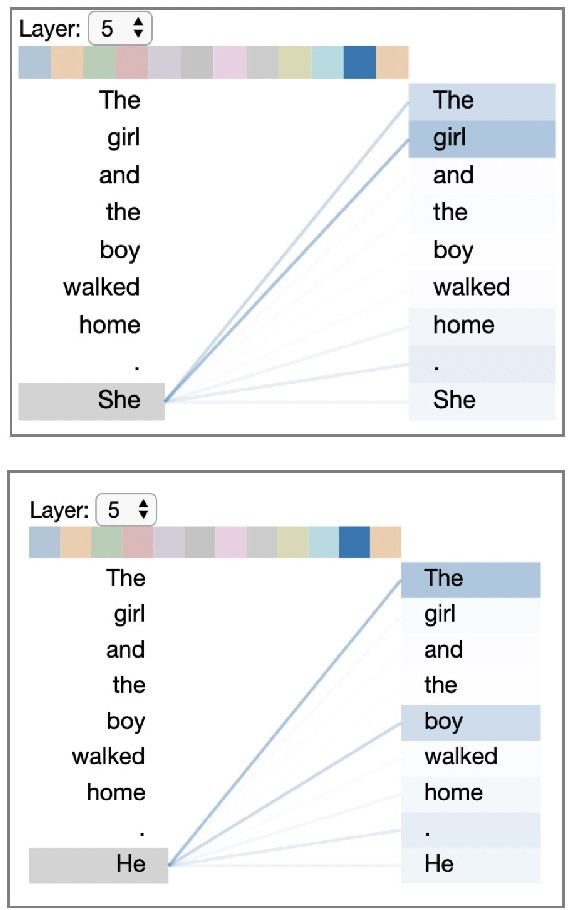
\includegraphics{img/attention_visualized.png}}
\caption{Visualization of attention in GTP-2 \cite{visualization_of_attention}}
\label{fig}
\end{figure}


\section{Training}

\section{Fazit}
Das ist ein Fazit



\printbibliography

\end{document}
